\documentclass[12pt]{article}

\title{Activity 5: Networking}
\author{Dr. Chris Mayfield}
\date{CS 101, Fall 2016}

%\ProvidesPackage{cspogil}

% fonts
\usepackage[utf8]{inputenc}
\usepackage[T1]{fontenc}
\usepackage{mathpazo}

% spacing
\usepackage[margin=2cm]{geometry}
\renewcommand{\arraystretch}{1.4}
\setlength{\parindent}{0pt}

% orphans and widows
\clubpenalty=10000
\widowpenalty=10000
\pagestyle{empty}

% figures and tables
\usepackage{graphicx}
\usepackage{multicol}
\usepackage{tabularx}
\usepackage{wrapfig}

% fixed-width columns
\usepackage{array}
\newcolumntype{L}[1]{>{\raggedright\let\newline\\\arraybackslash\hspace{0pt}}m{#1}}
\newcolumntype{C}[1]{>{\centering\let\newline\\\arraybackslash\hspace{0pt}}m{#1}}
\newcolumntype{R}[1]{>{\raggedleft\let\newline\\\arraybackslash\hspace{0pt}}m{#1}}

% include paths
\makeatletter
\def\input@path{{Models/}{../../Models/}}
\graphicspath{{Models/}{../../Models/}}
\makeatother

% colors
\usepackage[svgnames,table]{xcolor}
\definecolor{bgcolor}{HTML}{FAFAFA}
\definecolor{comment}{HTML}{007C00}
\definecolor{keyword}{HTML}{0000FF}
\definecolor{strings}{HTML}{B20000}

% table headers
\newcommand{\tr}{\bf\cellcolor{Yellow!10}}

% syntax highlighting
\usepackage{textcomp}
\usepackage{listings}
\lstset{
    basicstyle=\ttfamily\color{black},
    backgroundcolor=\color{bgcolor},
    numberstyle=\scriptsize\color{comment},
    commentstyle=\color{comment},
    keywordstyle=\color{keyword},
    stringstyle=\color{strings},
    columns=fullflexible,
    keepspaces=true,
    showlines=true,
    showstringspaces=false,
    upquote=true
}

% code environments
\newcommand{\java}[1]{\lstinline[language=java]{#1}}%[
\lstnewenvironment{javalst}{\lstset{language=java,backgroundcolor=}}{}
\lstnewenvironment{javabox}{\lstset{language=java,frame=single,numbers=left}\quote}{\endquote}

% PDF properties
\usepackage[pdftex]{hyperref}
\urlstyle{same}
\makeatletter
\hypersetup{
  pdftitle={\@title},
  pdfauthor={\@author},
  pdfsubject={\@date},
  pdfkeywords={},
  bookmarksopen=false,
  colorlinks=true,
  citecolor=black,
  filecolor=black,
  linkcolor=black,
  urlcolor=blue
}
\makeatother

% titles
\makeatletter
\renewcommand{\maketitle}{\begin{center}\LARGE\@title\end{center}}
\makeatother

% boxes [optional height]
\newcommand{\emptybox}[1][10em]{
\vspace{1em}
\begin{tabularx}{\linewidth}{|X|}
\hline\\[#1]\hline
\end{tabularx}}

% models
\newcommand{\model}[1]{\section{#1}\nopagebreak}
\renewcommand{\thesection}{Model~\arabic{section}}

% questions
\newcommand{\quest}[1]{\subsection*{Questions~ (#1)}}
\newcounter{question}
\newcommand{\Q}{\vspace{1em}\refstepcounter{question}\arabic{question}.~ }
\renewcommand{\thequestion}{\#\arabic{question}}

% sub-question lists
\usepackage{enumitem}
\setenumerate[1]{label=\alph*)}
\setlist{itemsep=1em,after=\vspace{1ex}}

% inline answers
\definecolor{answers}{HTML}{C0C0C0}
\newcommand{\ans}[1]{%
\ifdefined\Student
    \leavevmode\phantom{~~\textcolor{answers}{#1}}
\else
    ~~\textcolor{answers}{#1}
\fi}

% longer answers [optional height]
\newsavebox{\ansbox}
\newenvironment{answer}[1][4em]{
\nopagebreak
\begin{lrbox}{\ansbox}
\begin{minipage}[t][#1]{\linewidth}
\color{answers}
}{
\end{minipage}
\end{lrbox}
\ifdefined\Student
    \phantom{\usebox{\ansbox}}%
\else
    \usebox{\ansbox}%
\fi}


\begin{document}

\maketitle

The Internet is the underlying global communications network that supports the World Wide Web and many other applications. It consists of many different local networks that are connected together by various hardware devices.


% based on Model 3 of Activity 12 - Internet by Helen Hu
\model{How the Internet Works}

All devices connected to the Internet are assigned an \emph{IP address} made up of four numbers separated by dots (e.g., 70.42.251.42). Some are assigned a \emph{static} (permanent) IP address, whereas others are assigned a \emph{dynamic} (temporary) IP address. Since it's difficult for people to remember numbers, we typically use \emph{domain names} when referring to websites.

\begin{center}
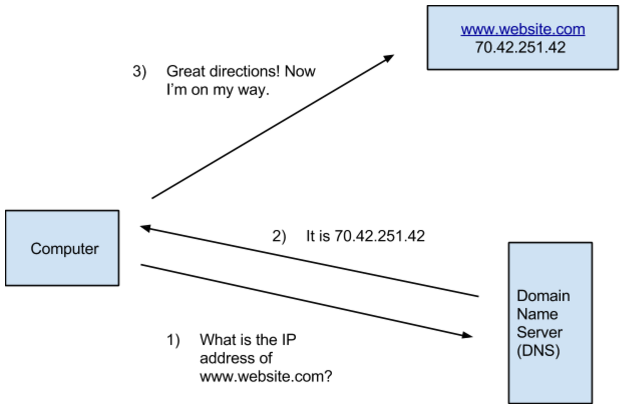
\includegraphics[width=0.75\textwidth]{dns.png}
\end{center}


\quest{15 min}


\Q Examine the above model.
\begin{enumerate}
\item What is the domain name in the above model?
\item What is the IP address given in the above model?
\item What is the binary version of the IP address in the above model?
\end{enumerate}


\Q Given that IP addresses are four 8-bit binary numbers, what is the largest possible IP address?

\begin{answer}
\end{answer}


\Q What is the function of a DNS Server?

\begin{answer}
\end{answer}


\Q Give examples of domain names that you like to visit (at least one for each person in your group).

\begin{answer}
\end{answer}


\Q How are domain names an example of an abstraction?

\begin{answer}
\end{answer}


\Q In your own words, describe the steps for retrieving a webpage (as provided by the above model).

\begin{answer}
\end{answer}


\Q Find each of your computer's IP address by typing ``Find My IP Address'' in Google. List all addresses for your team here.

\begin{answer}
\end{answer}


\Q Go to TCPIPutils.com and type in our college's url (\_\_\_\_\_.edu) into the search field.
Scroll down half-way down the page to ``IP-range/subnet''.
\begin{enumerate}
\item Identify the range of IP addresses used by your college.
\item Does the university have enough IP addresses for all students, faculty, and staff (and their multiple devices)? Explain your answer.
\end{enumerate}


% based on Model 4 of Activity 12 - Internet by Helen Hu
\model{Measuring Your Network}

Your network performance can be measured in two ways:
\begin{itemize}
\item \textbf{bandwidth} -- the rate at which data is downloaded or uploaded to a network (measured in bits per second (bps), Kilobits per second (Kbps) or Megabits per second (Mbps)
\item \textbf{latency} -- measure of time it takes a piece of data to reach its destination (measured in milliseconds)
\end{itemize}


\quest{10 min}


\Q Consider how good performance would be measured:
\begin{enumerate}
\item When measuring bandwidth, would good performance be a large number or a small number?
\item When measuring latency, would good performance be a large number or a small number?
\end{enumerate}


\Q Use CNET’s bandwidth tool to measure bandwidth here on campus (and later at home).
\begin{enumerate}
\item On campus
\item At home
\end{enumerate}


\Q Use this Ping tool to measure the average latency between the site and:
\begin{enumerate}
\item http://google.com
\item http://whitehouse.gov
\item Are there any websites you use that you find slow? Give that website and its latency:
\end{enumerate}


\Q Use Ookla’s Broadband map to explore bandwidth speeds in the US. Check for your home state (or where you attend school).
\begin{enumerate}
\item Which state in the US has the fastest average speed? Which state has the slowest? 
\item What is the difference between the fastest and slowest states?
\item You can also compare bandwidth speeds between countries using Ookla’s global map.  Which country has the fastest average speed? How does your country compare?
\end{enumerate}

\end{document}
